\documentclass[letterpaper,11pt]{article}
% Soporte para los acentos.
\usepackage[utf8x]{inputenc}
\usepackage[T1]{fontenc}    
% Idioma español.
\usepackage[spanish,mexico, es-tabla]{babel}
% Soporte de símbolos adicionales (matemáticas)
\usepackage{multirow}
\usepackage{amsmath}		
\usepackage{amssymb}		
\usepackage{amsthm}
\usepackage{amsfonts}
\usepackage{latexsym}
\usepackage{enumerate}
\usepackage{ragged2e}
% Soporte para la imágenes.
\usepackage{graphicx}
\usepackage{forest,array}
% Soporte para Tableaux
\usepackage{prooftrees}
% Modificamos los márgenes del documento.
\usepackage[lmargin=2cm,rmargin=2cm,top=2cm,bottom=2cm]{geometry}

\title{Universidad Nacional Autónoma de México \\
       Facultad de Ciencias \\
       Estructuras Discretas \\ 
       Tarea 1}
\author{Rubí Rojas Tania Michelle \\
        taniarubi@ciencias.unam.mx \\
        \# cuenta: 315121719}
\date{1 de septiembre de 2017}

\begin{document}
\maketitle

\begin{enumerate}
    % Ejercicio 1.
    \item Demuestre que las siguientes expresiones están bien formadas.    
    
    \begin{itemize}
        % Ejercicio 1.1
        \item $- ((a + b) * c) + 1$

        \textsc{Solución:} Para mostrar que la expresión está bien formada,
        daremos su respectivo árbol de derivación.

        \begin{center}
            \begin{forest}  
                [S, for tree={parent anchor=south, child anchor=north} 
                    [E, for tree={parent anchor=south, child anchor=north}
                        [E 
                            [$\rhd$ [-]] 
                                [E 
                                    [E 
                                        [(] 
                                            [E 
                                                [E 
                                                    [(] 
                                                        [E 
                                                            [E [$\text{var}$ [a]]] 
                                                                [$\diamond$] 
                                                                    [E [$\text{var}$ [b]]]] 
                                                            [)]] 
                                                        [$\diamond$ [*]] 
                                                    [E [$\text{var}$ [c]]]] 
                                                [)]] 
                                    [$\diamond$ [+]] 
                                        [E [$\text{const}$ [1]]]]]]]
            \end{forest}
        \end{center}

        \newpage
        % Ejercicio 1.2
        \item $((p → q) \land (r → s)) \lor r$

        \textsc{Solución:} Para mostrar que la expresión está bien formada, 
        daremos su respectivo árbol de derivación.

        \begin{center}
            \begin{forest}
                [S, for tree={parent anchor=south, child anchor=north}
                    [E, for tree={parent anchor=south, child anchor=north}
                        [E 
                            [(] 
                                [E 
                                    [E 
                                        [(] 
                                            [E 
                                                [E [$\text{var}$ [p]]] 
                                                    [$\diamond$ [$→$]] 
                                                        [E [$\text{var}$ [q]]]]
                                                [)]] 
                                        [$\diamond$ [$\land$]] 
                                            [E 
                                                [(] 
                                                    [E 
                                                        [E [$\text{var}$ [r]]] 
                                                            [$\diamond$ [$→$]] 
                                                                [E [$\text{var}$ [s]]]] 
                                                        [)]]] 
                                    [)]] 
                            [$\diamond$ [$\lor$]] 
                                [E [$\text{var}$ [r]]]]]
            \end{forest}
        \end{center}
    \end{itemize}

    % Ejericicio 2.
    \item Determine cuáles de las siguientes oraciones son proposiciones 
    atómicas, cuáles son proposiciones no atómicas y cuáles no son 
    proposiciones. Justifique su respuesta. 

    \begin{itemize}
        % Ejercicio 2.1
        \item[a)] El grito de Dolores, en $1810$, sentó las bases para la 
        independencia de México.

        \textsc{Solución:} Esta oración es una proposición ya que puede 
        calificarse como falso o verdadero, y es atómica porque no puede 
        descomponerse en más proposiciones debido a que no contiene conectivos 
        lógicos.

        % Ejercicio 2.2
        \item[b)] Para pasar el examen es necesario que los alumnos estudien, 
        hagan la tarea y asistan a clase.

        \textsc{Solución:} Esta oración es una proposición ya que puede 
        calificarse como falso o verdadero, y es compuesta porque puede 
        descomponerse en más proposiciones debido a que contiene los conectivos
        lógicos \textit{es necesario}, e $y$.

        % Ejercicio 2.3
        \item[c)] $a^{3} + 3a^{2}b + 3ab^{2} + a^{3}$

        \textsc{Solución:} Esta oración no es una proposición ya que no puede 
        calificarse como falso o verdadero.

        % Ejercicio 2.4
        \item[d)] $x \neq y$. (Donde el operador binario $\neq$ evalúa a 
        \textbf{verdadero} si $x$ es distinto de $y$ y a \textbf{falso} si 
        $x$ es igual a $y$)

        \textsc{Solución:} Esta oración es una proposición ya que puede 
        calificase como falso o verdadero (gracias a su operador binario), y es 
        atómica porque no puede descomponerse en más proposiciones debido a que 
        no contiene conectivos lógicos. 

        % Ejercicio 2.5
        \item[e)] Asgard es el mundo de los AEsir y en Svartálfaheim habitan los 
        Svartalfar.

        \textsc{Solución:} Esta oración es una proposción ya que puede 
        calificarse como falso o verdadero, y es compuesta porque contiene el 
        conectivo lógico $y$. 
    \end{itemize}

    \newpage
    % Ejercicio 3.
    \item De los incisos de la pregunta anterior que son proposiciones, exhiba
    una traducción al lenguaje de la lógica proposicional.

    \begin{itemize}
        \item[a)] $p$ \\ 
        Donde $p:$ el grito de Dolores, en $1810$, sentó las bases para la 
        independencia de México.

        \item[b)] $p → (q \land r \land s)$ \\ 
        Donde 
        \begin{itemize}
            \item $p:$ los alumnos pasan el examen.
            \item $q:$ los alumnos estudian.
            \item $r:$ los alumnos hacen la tarea.
            \item $s:$ los alumnos asisten a clase.
        \end{itemize}
    
        \item[d)] $p$ \\ 
        Donde $p: \; x \neq y$
        \item[e)] $p \land q$ \\ 
        Donde 
        \begin{itemize}
            \item $p:$ Asgard es el mundo de los AEsir.
            \item $q:$ en Svartálfaheim habitan los Svartalfar.
        \end{itemize}
    \end{itemize}

    % Ejercicio 4.
    \item Coloque los paréntesis en las siguientes expresiones de acuerdo a la 
    precedencia y asociatividad de los operadores, sin preocuparse por la
    evaluación de la expresión.

    \begin{itemize}
        % Ejercicio 4.1
        \item[a)] $-b + b * * 2 - 4 \cdot a \cdot c / 2 \cdot a$ 
        
        \textsc{Solución:} 
        $(((-b) + (b * * 2)) - ((((4 \cdot a) \cdot c) / 2) \cdot a))$ 

        % Ejercicio 4.2
        \item[b)] $p \land q \lor r → s ↔ p \lor q$

        \textsc{Solución:} $((((p \land q) \lor r) → s) ↔ (p \lor q))$

        % Ejercicio 4.3
        \item[c)] $a < b \land b < c → a < b$

        \textsc{Solución:} $a < b \land b < c → a < b$

        % Ejercicio 4.4
        \item[d)] $a \cdot b -a \cdot c ↔ a > 0 \land b > c$
        
        \textsc{Solución:} 
        $(((a \cdot b) - (a \cdot c)) ↔ ((a > 0) \land (b > c)))$
    \end{itemize}

    % Ejercicio 5.
    \item Ejecute las siguientes sustituciones textuales simultáneas, fijándose
    bien en la colocación de los paréntesis. Quite los paréntesis que son 
    redundantes.

    \begin{itemize}
        % Ejercicio 5.1
        \item[a)] $5x + 3y * a - 4y[y := x]$ 

        \textsc{Solución:} La sustitución se aplica a la expresión más cercana,
        que en este caso es $4y$.
        \begin{align*} 
            5x + 3y * a - 4y[y := x]
            =& \; 5x + 3y * a - 4(x) \\
            =& \; 5x + 3y * a - 4x
        \end{align*}

        % Ejercicio 5.2
        \item[b)] $(5x + 3y * a - 4y)[y := x]$

        \textsc{Solución:} La sustitución de aplica a toda la expresión.
        \begin{align*}
            (5x + 3y * a - 4y)[y := x]
            =& \; (5x + 3(x) * a - 4(x)) \\
            =& \; 5x + 3x * a - 4x    
        \end{align*}

        % Ejercicio 5.3
        \item[c)] $(5x + 3y * a - 4y)[y, \; x := x, \;y]$

        \textsc{Solución:}
        \begin{align*}
            (5x + 3y * a - 4y)[y, \; x := x, \;y]
            =& \; (5(y) + 3(x) * a - 4(x)) \\ 
            =& \; 5y + 3x * a - 4x
        \end{align*}

        % Ejercicio 5.4
        \item[d)] $(5x + 3y * a - 4y)[y := x][x := 3]$

        \textsc{Solución:}
        \begin{align*}
            (5x + 3y * a - 4y)[y := x][x := 3]
            &= \; (5x + 3(x) * a - 4(x))[x :=3] \\ 
            &= \; (5(3) + 3((3))) * a - 4((3)) \\ 
            &= \; 15 + 9 * a - 12
        \end{align*}
    \end{itemize}

    % Ejercicio 6.
    \item Para las siguientes expresiones, determine a qué esquema pertenecen,
    dé el rango y conectivo principal. Justifique su respuesta.

    \begin{itemize}
        % Ejercicio 6.1
        \item[a)] $((p \land q) \lor (r → s)) → r$

        \textsc{Solución:} Esta expresión pertenece al esquema condicional, y 
        para justificarlo mostraremos la sucesión de sustituciones textuales 
        que se fueron realizando: 

        \begin{align*}
            (p → q)[p, \; q := a \lor b, \; r][a, \; b := p \land q, \; r → s]
            =& ((a \lor b) → r)[a, \; b := p \land q, \; r → s] \\
            =& (((p \land q) \lor (r → s)) → r) \\
            =& ((p \land q) \lor (r → s)) → r
        \end{align*}

        Por lo tanto, el conectivo principal es $→$, de donde su rango izquierdo 
        es $((p \land q) \lor (r → s))$ y su rango derecho es $r$.

        % Ejercicio 6.2
        \item[b)] $p \lor q → r → s ↔ t$

        \textsc{Solución:} Primero, le colocamos paréntesis a la expresión 
        según la precedencia y la asociatividad de los conectivos.
        
        \begin{center}
            $(((p \lor q) → (r → s)) ↔ t)$
        \end{center}

        Así, esta expresión pertenece al esquema condicional, y para 
        justificarlo mostraremos la sucesión de sustituciones textuales que se 
        fueron realizando:

        \begin{align*}
            (p ↔ q)[p, \; q := a → b, \; t][a, \; b := p \lor q, \; r → s]
            =& ((a → b) ↔ t)[a, \; b := p \lor q, \; r → s] \\ 
            =& (((p \lor q) → (r → s)) ↔ t)
        \end{align*}

        Por lo tanto, el conectivo principal es $↔$, de donde su rango derecho 
        es $t$ y su rango izquierdo es $((p \lor q) → (r → s))$.
    \end{itemize}

    \newpage
    % Ejercicio 7.
    \item Para cada una de las expresiones del ejercicio anterior, construya
    los árboles de análisis sintáctico.

    \begin{itemize}
        \item[a)] $((p \land q) \lor (r → s)) → r$

        \textsc{Solución:}
        \begin{center}
            \begin{forest}
                [S, for tree={parent anchor=south, child anchor=north}
                    [E, for tree={parent anchor=south, child anchor=north}
                        [E 
                            [(] 
                                [E 
                                    [E 
                                        [(] 
                                            [E 
                                                [E [$\text{var}$ [p]]] 
                                                    [$\diamond$ [$\land$]] 
                                                        [E [$\text{var}$ [q]]]] 
                                                [)]] 
                                        [$\diamond$ [$\lor$]] 
                                            [E 
                                                [(] 
                                                    [E 
                                                        [E [$\text{var}$ [r]]] 
                                                            [$\diamond$ [$→$]] 
                                                                [E [$\text{var}$ [s]]]] 
                                                        [)]]] 
                                    [)]] 
                            [$\diamond$ [$→$]] 
                                [E [$\text{var}$ [r]]]]]
            \end{forest}
        \end{center}

        \item[b)] $p \lor q → r → s ↔ t$

        \textsc{Solución:}
        \begin{center}
            \begin{forest}
                [S, for tree={parent anchor=south, child anchor=north}
                    [E, for tree={parent anchor=south, child anchor=north}
                        [E 
                            [(] 
                                [E 
                                    [E 
                                        [(] 
                                            [E 
                                                [E [$\text{var}$ [p]]] 
                                                    [$\diamond$ [$\lor$]] 
                                                        [E [$\text{var}$ [q]]]] 
                                                [)]] 
                                        [$\diamond$ [$→$]] 
                                            [E 
                                                [(] 
                                                    [E 
                                                        [E [$\text{var}$ [r]]] 
                                                            [$\diamond$ [$→$]] 
                                                                [E [$\text{var}$ [s]]]] 
                                                        [)]]] 
                                    [)]] 
                            [$\diamond$ [$↔$]] 
                                [E [$\text{var}$ [t]]]]]
            \end{forest}
        \end{center}
    \end{itemize}

    \newpage
    % Ejercicio 8.
    \item Llene las partes que faltan y escriba en qué consiste la expresión 
    $E$.
    \begin{itemize}
        \item[a)] \;

        \item[b)] 
    \end{itemize}

    % Ejercicio 9.
    \item Utilizando únicamente la tabla de equivalencias dada en clase, 
    demuestre las siguientes equivalencias lógicas mediante razonamiento 
    ecuacional. Justifique cada paso.

    \begin{itemize}
        % Ejercicio 9.1
        \item[a)] $(A \lor B) → Q ≡ (A → Q) \land (B → Q)$ 
        \begin{proof}
            \begin{align*}
                (A \lor B) → Q 
                ≡& \; \neg (A \lor B) \lor Q  
                && \text{equivalencia de $→$} \\
                ≡& \; (\neg A \land \neg B) \lor Q 
                && \text{De Morgan} \\ 
                ≡& \; (\neg A \lor Q) \land (\neg B \lor Q)
                && \text{distributividad} \\ 
                ≡& \; (A → Q) \land (B → Q)
                && \text{equivalencia de $→$} 
            \end{align*}
        \end{proof}

        % Ejercicio 9.2
        \item[b)] $(A \land B) → Q ≡ (A → Q) \lor (B → Q)$ 
        \begin{proof}
            \begin{align*}
                (A \land B) → Q 
                ≡& \; \neg (A \land B) \lor Q
                && \text{equivalencia de $→$} \\ 
                ≡& \; (\neg A \lor \neg B) \lor Q
                && \text{De Morgan} \\
                ≡& \; (\neg A \lor \neg B) \lor (Q \lor Q)
                && \text{idempotencia} \\ 
                ≡& \; (\neg A \lor Q) \lor (\neg B \lor Q)
                && \text{distributividad} \\
                ≡& \; (A → Q) \lor (B → Q)
                && \text{equivalencia de $→$}
            \end{align*}
        \end{proof}

        % Ejercicio 9.3
        \item[c)] $(A \land B) → Q ≡ A → (B → Q)$
        \begin{proof}
            \begin{align*}
                (A \land B) → Q 
                ≡& \; \neg (A \land B) \lor Q
                && \text{equivalencia de $→$} \\ 
                ≡& \; (\neg A \lor \neg B) \lor Q
                && \text{De Morgan} \\ 
                ≡& \; \neg A \lor (\neg B \lor Q)
                && \text{asociatividad} \\ 
                ≡& \; A → (B → Q)
                && \text{equivalencia de $→$}
            \end{align*}
        \end{proof}
    \end{itemize}

    % Ejercicio 10.
    \item Para cada una de las siguientes fórmulas, determine si son o no 
    satisfacibles. En caso de serlo, muestre un modelo para cada una de ellas,
    y en caso de no serlo, demuestre que cada estado evalúa a falso.

    \begin{itemize}
        % Ejercicio 10.1
        \item[a)] $(P \lor Q) \land \neg P \land \neg Q$ 

        \textsc{Solución:} La fórmula no es satisfacible. Para demostrar que 
        cada estado evalúa a falso, mostraremos su respectiva tabla de verdad.

        \begin{center}
            \centerline{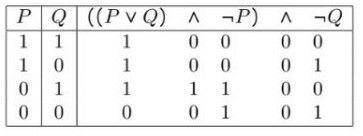
\includegraphics[scale=0.7]{tabla.jpg}}
        \end{center}

        % Ejercicio 10.2
        \item[b)] $(\neg P \lor Q) → ((P \land R) ↔ ((S \land T) → (U \lor P)))$

        \textsc{Solución:} La fórmula es satisfacible. El modelo $\mathcal{I}$
        tal que $\mathcal{I}(P) = 1$, $\mathcal{I}(Q) = \mathcal{I}(R) = 
        \mathcal{I}(S) = \mathcal{I}(T) = \mathcal{I}(U) = 0$ hace 
        que la expresión evalúe a verdadero.
    \end{itemize}

    % Ejercicio 11. 
    \item Decida si los siguientes conjuntos son satisfacibles. Justifique 
    su respuesta.

    \begin{itemize}
        % Ejercicio 11.1
        \item $\Gamma = \{p → q, \; p \lor r \land s, \; q → t\}$

        \textsc{Solución:} 
        % Ejercicio 11.2
        \item $\Gamma = \{p \lor q \lor r, \; \neg (r \lor \neg s), \; s ↔ t, \;
                          p → \neg t, \; q → (p \lor \neg t)\}$        
    \end{itemize}

    % Ejercicio 12.
    \item Para los siguientes argumentos, decida si son correctos y en caso de 
    no serlo dé una interpretación que haga verdaderas a las premisas y falsa 
    a la conclusión.

    \begin{itemize}
        % Ejercicio 12.1
        \item $p → q, \; p \lor r, \; \neg (r \land s), \; /∴ (p → q) → 
               (q \lor \neg s)$
        % Ejercicio 12.2
        \item $p \lor q, \; \neg (p \land r), \; \neg q \; /∴ r → s$
    \end{itemize}

    % Ejercicio 13.
    \item Construya las siguientes derivaciones.

    \begin{itemize}
        % Ejercicio 13.1
        \item $p \land (\neg r \land \neg w), \; l, \; r \land z ⊢ \neg r 
               \land (l \land z)$
        % Ejercicio 13.2
        \item $p \lor \neg(r \lor s), \; r, \; l → \neg p ⊢ \neg l$
        % Ejercicio 13.3
        \item $⊢(p → q) → (p \lor q → q)$
    \end{itemize}

    % Ejercicio 14.
    \item Construya la derivación del siguiente argumento para demostrar que es 
    correcto.

    Si procastinas en Helheim o en Asgard, entonces eres un AEsir. Procastinas 
    en Helheim. Pero, ser gobernado por Odín, es necesario para ser un AEsir. 
    Por lo tanto, eres gobernado por Odín o procastinas en Asgard.

    \begin{proof}
        Primero, transformamos el argumento a lenguaje de lógica proposicional.
        Asignamos las siguientes variables proposicionales:

        \begin{itemize}
            \item $p:$ Procastinas en Helheim.
            \item $q:$ Procastinas en Asgard.
            \item $r:$ Eres un AEsir.
            \item $s:$ Eres gobernado por Odín.
        \end{itemize}

        Así, el argumento a verificar es: $(p \lor q) → r, \; p, \; r → s$
        $/∴ \; s \lor q$. 

        Entonces
        \begin{align*}
            1.& \; \; (p \lor q) → r
            && \text{Premisa} \\ 
            2.& \; \; p
            && \text{Premisa} \\
            3.& \; \; r → s
            && \text{Premisa} \\ 
            4.& \; \; p \lor q
            && \text{I$\lor$ $2$} \\ 
            5.& \; \; r
            && \text{MP $4, 1$} \\ 
            6.& \; \; s
            && \text{MP $5, 3$} \\ 
            7.& \; \; s \lor q
            && \text{I$\lor$ $6$}
        \end{align*}

        Por lo tanto, el argumento es correcto.
    \end{proof}

    % Ejercicio 15.
    \item Usando Tableaux, determine la correctud del siguiente argumento.

    \begin{center}
        $(P \lor Q) → R, \; P, \; R → T \; /∴ T \lor Q$
    \end{center}

    \textsc{Solución:} Para determinar la correctud del argumento, debemos 
    comprobar que la siguiente fórmula es una tautología

    \begin{center}
        $(((P \lor Q) → R) \land P \land (R → T)) → (T \lor Q)$
    \end{center}

    Para ello, debemos constuir el Tableaux para la negación de la fórmula 
    anterior, es decir, 

    \begin{center}
        $((\neg P \land Q) \lor R) \land P \land (\neg R \lor T) \land 
        \neg T \land \neg Q$
    \end{center}

    Así, 
    \begin{center}
        \begin{prooftree}{}
            [(\neg P \land Q) \lor R, checked
            [\neg R \lor T, checked
            [P, checked
            [\neg T, checked
            [\neg Q
                [\neg R, checked, just={ext. de $\beta$ en $2$}
                    [\neg P \land Q, checked, just={ext. de $\beta$ en $1$} 
                        [\neg P, close={3,8}, just={ext. de $\alpha$ en $7$}]]  
                    [R, checked, close={6,7}]] 
                [T, checked, close={4,6}]]]]]]
        \end{prooftree}
    \end{center}

    Como el Tableaux es cerrado, eso significa que la fórmula es una tautología,
    y por lo tanto, el argumento es correcto.

    % Ejercicio 16.
    \item Usando Tableaux, demuestre que la siguiente fórmula es una tautología.

    \begin{center}
        $p \lor (\neg p \land q) → p \lor q$
    \end{center}

    \begin{proof} 
        Debemos construir el Tableaux de la negación de la fórmula, es decir, 
        hay que constuir el Tableaux para
        
        \begin{center}
            $p \lor (\neg p \land q) \land \neg p \land \neg q$
        \end{center}
        
        Así, 
        \begin{center}
            \begin{prooftree}{}
                [p \lor (\neg p \land q), checked
                [\neg p, checked
                [\neg q, checked
                    [p, checked, close={2,4}, just={ext. de $\beta$ en $1$}] 
                        [\neg p \land q, checked 
                        [q, checked, close={3,4}, just={ext. de $\alpha$ en $4$}]]]]]
            \end{prooftree}
        \end{center}

    Como el Tableaux es cerrado, eso significa que la fórmula es una 
    tautología.

    \end{proof}
\end{enumerate}

\end{document}
